\chapter{System Design}

This section is based on the final product of the project. Any compatibility or deployment issues that have been mentioned will be discussed in the system evaluation section.

\section{CI/CD Design and Implementation}
GitHub Actions is used as the CI/CD tool in this project. Workflow files (.yml or .yaml) that automate tests, deployment, etc. are assigned using GitHub Actions. It is possible to run the workflow automatically after certain GitHub events like commit push. A green tick or a red cross will be shown beside the commit in the repository to indicate if the workflow has been completed successfully.

Workflow files can be designed manually or by using recommended workflows on GitHub such as Jekyll or readily made template like JupyterLite. In this project, the pipeline is designed manually. Refer to Figure~\ref{image:full-workflow} in Appendix~\ref{appendix:CICD} for the full workflow code or redirect to the GitHub repository page \href{https://github.com/gabhang/final-year-project}{here}.

The workflow is triggered whenever a commit is pushed to the main branch. The workflow has one job named "build" that will run on an Ubuntu operating system that has four steps. The first step checks out from the repository for automation. The second step sets up the Node.js environment with version 18. The third step installs the necessary dependencies for the project using \texttt{npm install}. The fourth step runs the tests to ensure that the website's features are working correctly. Finally, the last step in the workflow deploys the application to Heroku using the \textit{akhileshns/heroku-deploy} action with the Heroku API key the app name and the email of the account. The Heroku API key is stored in GitHub secrets and is accessed through the \$\{\{ secrets.HEROKU\textunderscore API\textunderscore KEY \}\} variable.

Overall, this workflow ensures that the website's features work perfectly by building, testing, and deploying the application automatically in response to changes in the main branch.

The \texttt{npm test} in the workflow file runs the tests automatically from the directory. The test file was design using Supertest and Jest to test out CRUD API. The code snippet from Figure~\ref{image:test-create} below tests the functionality of a create functionality, specifically, the \texttt{createGrade} function that creates a new student record. It sends a HTTP POST request to the \textit{/createGrade} endpoint with test data and expects a response status code of 200 and a response message of 'Student Grade Added'. It stores the ID of the newly created student record in a variable called \texttt{testId} to test out other functionalities. This test case ensures that the createGrade function is able to create new student records without errors.

\begin{figure}[h!]
    \centering
    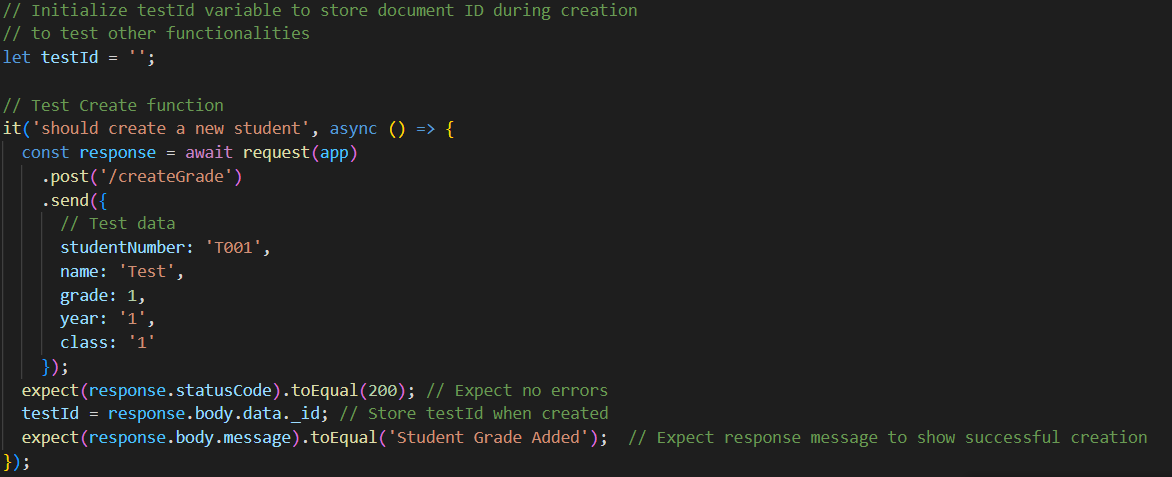
\includegraphics[width=0.9\textwidth]{images/test-create.png}
    \caption{Test Create Functionality}
    \label{image:test-create}
\end{figure}

After ensuring the application is working as expected by running the test suite, the workflow uses Heroku to deploy the application. It is vital to note that \textit{Procfile} is included in the directory as it specifies the commands that are executed by the application on startup, and the server will be started up in this context. The build file from the client side is duplicated to the server side as the server will be run first and after building the server, the Heroku post-build is used to run the build file to show the frontend. Figure~\ref{image:heroku-build} in Appendix~\ref{appendix:CICD} shows that \texttt{heroku-postbuild} is added under the script in package-json.

\section{MongoDB Database Design}

For this project, there is a collection in the database called \textit{grades} with the following structure:

\begin{table}[ht]
    \centering
    \begin{tabular}{|p{3.5cm}||p{3cm}||p{5.5cm}|}
    \hline
    \textbf{Field} & \textbf{Datatype} & \textbf{Special Conditions} \\
    \hline \hline
    \textunderscore id  & ObjectId & Auto-generated by database \\
    \hline
    studentNumber  & String & Required \\
    \hline
    name & String & Required \\
    \hline
    grade & String & Required \\
    \hline
    year & String & Required \\
    \hline
    class & String & Required \\
    \hline
    \end{tabular}
    \linebreak
        \caption{MongoDB Structure}
        \label{tab:mongodbstruc}
\end{table}

\section{MERN Stack}
As discussed previously in methodology with reference to Figure~\ref{appendix:mern} in Appendix~\ref{appendix:mern}, The database used for the system is MongoDB, the frontend or the webpage is developed using React.js and the backend or the server is built using Node.js with Express.js framework. The CRUD functionalities that are implemented in the student grade system for this project are as follows:

\begin{itemize}
\item Create: Add a student with grades and other information.
\item Read: Get all students' information and filter certain categories of students.
\item Update: Update student grades and/or information.
\item Delete: Delete a student.
\end{itemize}

The above functionalities are designed as APIs in the backend with the frontend used for interaction and the database utilized for managing the data.
